%%%%%%%%%%%%%%%%%%%% author.tex %%%%%%%%%%%%%%%%%%%%%%%%%%%%%%%%%%%
%
% sample root file for your "contribution" to a proceedings volume
%
% Use this file as a template for your own input.
%
%%%%%%%%%%%%%%%% Springer %%%%%%%%%%%%%%%%%%%%%%%%%%%%%%%%%%


\documentclass{svproc}
%
% RECOMMENDED %%%%%%%%%%%%%%%%%%%%%%%%%%%%%%%%%%%%%%%%%%%%%%%%%%%
%

% to typeset URLs, URIs, and DOIs
\usepackage{url}
\usepackage[backend=biber]{biblatex}
\usepackage{graphics}
\usepackage{multirow}
\usepackage{caption}
\usepackage{subcaption}

\def\UrlFont{\rmfamily}
\bibliography{bibliography}

\begin{document}
\mainmatter              % start of a contribution
%
\title{BellChat: An inclusive web application for messaging}
%
\titlerunning{BellChat}  % abbreviated title (for running head)
%                                     also used for the TOC unless
%                                     \toctitle is used
%
%\author{Ivar Ekeland\inst{1} \and Roger Temam\inst{2}
%Jeffrey Dean \and David Grove \and Craig Chambers \and Kim~B.~Bruce \and Elsa Bertino}
%
\author{Gleiston Guerrero-Ulloa\inst{1,2} (0000-0001-5990-2357) \and Víctor Romero-Castro\inst{1} (0000-0003-4920-1009) \and Janer Torrales-Peralta\inst{1} (0000-0001-6587-9587)  \and Tyrone Tocta-Bonilla\inst{1} (0000-0002-5812-0617) \and Orlando Erazo\inst{1} (0000-0001-5642-9920)}
\authorrunning{Gleiston Guerrero-Ulloa et al.} % abbreviated author list (for running head)
%
%%%% list of authors for the TOC (use if author list has to be modified)
%\tocauthor{Ivar Ekeland, Roger Temam, Jeffrey Dean, David Grove, Craig Chambers, Kim B. Bruce, and Elisa Bertino}
\tocauthor{Gleiston Guerrero-Ulloa, Víctor Romero-Castro, Janer Torrales-Peralta, Tyrone Tocta-Bonilla, and Orlando Erazo}

%
\institute{State Technical University of Quevedo, Quevedo, 120301 Los Ríos, Ecuador,\\
\email{\{gguerrero,victor.romero2016,janer.torrales2016,tyrone.tocta2016, oerazo\}@uteq.edu.ec},\\ WWW home page:
\texttt{https://www.uteq.edu.ec/} \and
University of Granada, Granada, 18071 Granada, Spain,\\
	\email{gleiston@correo.ugr.es},\\ WWW home page:
	\texttt{https://www.ugr.es/}}
%\institute{Princeton University, Princeton NJ 08544, USA,\\
%\email{I.Ekeland@princeton.edu},\\ WWW home page:
%\texttt{http://users/\homedir iekeland/web/welcome.html}
%\and
%Universit\'{e} de Paris-Sud,
%Laboratoire d'Analyse Num\'{e}rique, B\^{a}timent 425,\\
%F-91405 Orsay Cedex, France}

\maketitle              % typeset the title of the contribution

\begin{abstract}
Minority groups of web users, such as people with disabilities and elderly people, are limited in their ability to communicate through chat applications. Social networks are especially used in communication among their users. However, social networks such as Facebook (Messenger), Twitter and WhatsApp are not adapted for these groups, and therefore, they do not fully meet the needs for which they were created. Moreover, for people with disabilities to use web-based messaging applications, they are required to use third-party tools, such as screen readers. For these reasons, this paper presents BellChat, a responsive web application for communication between everybody, adapted for people with disabilities. BellChat converts text messages into speech, or speech messages into text, depending on the disability of the user. BellChat was developed following the Scrum framework with adaptations to very small groups. The roles, the modality of work and the meetings frequency were adapted to the project.
% We would like to encourage you to list your keywords within
% the abstract section using the \keywords{...} command.
%\keywords{computational geometry, graph theory, Hamilton cycles}

\keywords{Visual impairment, Hearing impairment, web accessibility, Text-to-speech, Speech-to-text}

\end{abstract}
%
\section{Introducción}
%
Although inclusivity goes beyond accessibility, its basis is accessibility. An inclusive web application must first be an accessible web application. This means that an application should be thought of from the design to the building and deployment as an application that is accessible to all people without exception \cite{WCAG202012}. To achieve this goal, the Web Accessibility Initiative (WAI) of the World Wide Web Consortium (W3C) has been established to raise awareness of universal accessibility \cite{W3C2022}. The WAI provides developers with guidelines that can help make web pages widely accessible \cite{Shawar2015}. Considering that websites are designed to serve different purposes such as information, entertainment, advertising, to name a few, and that to achieve this goal they present a wide range of information to meet user needs, they must be accessible to everybody. However, most of these websites do not comply with the web accessibility standards designed by the W3C, making it difficult for part of the population to access to web content\cite{Broccia2020}.

The Web was created with the purpose of giving access to all people without exception. Therefore, the Web is the place where everybody should feel their full right to equality, regardless of their conditions or disabilities \cite{Pelzetter2020}. However, what happen with people with disabilities? In general, disability encompasses impairments, limitations, and other factors that affect certain bodily functions or prevent from performing common activities, among other problems. There are several types of disabilities, such as physical, sensory (visual, hearing), intellectual and multiple disabilities \cite{Lister2020}. It is very common to find websites that are not adapted for people with disabilities; for example, they do not have their own content reader, or they do not have a voice command interface. Likewise, not all websites take care of people with hearing disabilities, i.e., the voice files generally do not have the transcription of the content into text to allow for people with hearing disabilities understanding the content \cite{DominguezVila2018}.

Given these disadvantages, people with visual or hearing impairments face the difficult task of using communication resources. Visually impaired people lessen this difficulty by using screen readers provided by third parties\cite{Morris2018}, while tools to reduce the difficulty faced by the hearing-impaired people are poorly suited for instant transcription of voice messages by downloading the message and uploading it to the applications for transcription. Some of these tools and the most popular ones can be found at González \cite{Gonzalez2021}. Two authors of this work share with hearing impaired people, who have shared with them that. When they receive voice messages (by mistake or due to ignorance of the senders), they must ask for help from third parties to know the content. This situation is also affirmed by  Pereira \cite{Pereira2010}. In addition, these two groups of people with disabilities are joined by older adults who, due to their condition, are diminished in their abilities, and therefore do not enjoy all the benefits offered by the evolution of the functionalities of web applications for communication \cite{Lister2020}.

Communication between human beings is what makes people live in society. Currently around 3.4 billion users actively use social media platforms daily for an average of 2.5 hours \cite{Arya2022}. Social media has become an effective means of communication between people, including for companies with their customers. However, the lack of inclusive platforms may make people with disabilities feel excluded \cite{Arora-Jonsson1687809}. As a contribution to achieve the inclusion of this group of people, this paper presents BellChat, a responsive web application that ensures accessibility to the greatest number of people, regardless of their conditions (visual, hearing, physical). Its virtual assistant ensures interaction between the user and the application. It enables the actions allowed on each page to be performed by voice commands; it also allows any user to send messages in any format to people with or without disabilities. In addition, to reach as many people as possible, keyboard commands have been implemented for those who have problems with the mouse and for people who may have problems with the pronunciation of voice commands \cite{OnayDurdu2022,Wang2017}.
BellChat implements the W3C standards and complies with the success criteria to make web pages accessible to as many people as possible \cite{WCAG202012}. Based on these standards, the communication between people with and without disabilities is facilitated and communication accessibility problems are reduced. Other communication websites comply with certain W3C standards, but they do not achieve the objective of maximizing the number of people because they do not provide ease of use for people with disabilities. Thus, this document details the development and evaluation of BellChat.

\section{Related Work}

In digital libraries, such as WOS (Web of Science), ACM, IEEE, Scopus, and Elsevier, few papers have been found on the development of accessible web applications. However, there are some articles that deal with the evaluation of web accessibility in public interest websites.
Among the works that present the development of accessible web applications, we can find Web-ALAP, a web-based application for writing mathematical documents in LaTeX developed by  \cite{Arooj2020}. Web-ALAP supports users with low vision through assistive functions and the manifestation of error indications by voice. To support users with the same disability, In \cite{Lee2020}, introduce TableView, which focuses on solving the problem of users with low vision who have difficulty using the on-screen magnifier. TableView extracts content and information from the page and presents it in a more compact form to make the most of the expanded space. Despite their contribution, these works are focused on a specific problem: people with low vision.

Among the works that have been concerned with people with profound deafness problems, Lyall and collaborators developed a smartphone application that recognised six sentences dictated by doctors for post-operative patients \cite{Lyall2016}. These messages, delivered by voice by doctors, were converted to text to be read by the patients. The results shown in this work., with a clear extension, can be used for telephone conversations and even in face-to-face conversations between people without disabilities and with hearing loss.

Along the same lines, we find the work of \cite{Shadiev2014}, in which they apply speech-to-text technology in a virtual classroom. Their results were a motivation to propose BellChat. Although \cite{Shadiev2014} applies it directly, BellChat does it in a deferred way, in text messages and speech-to-text over voice files. Moreover, a mobile application that enables communication between hearing impaired and non-disabled people (or those who do not understand sign language) was presented by Ali and Aydah \cite{Ali2012} which, via Bluetooth, allows for exchanging information over short distances.

In \cite{Alsaif2017} present a very useful application for people with speech problems. It predicts through statistics the words that could be pronounced in a conversation. In addition to converting text to speech, the system provides different categories of frequently used phrases that are labelled with a representative image for ease of use. The user can also add images to the system and record the human voice or use the automatic text-to-speech synthesiser. The limitation of this application is that it is smartphone-only and converts speech to text and text-to-speech using only Arabic language.

On the other hand, one of the activities that help make websites accessible is accessibility evaluation. Academic websites and government websites have been targeted by evaluators. For example, Sala et al., \cite{Sala2020} conducted a user study to evaluate five Spanish governmental websites. This study involved five people with low vision out of a total of ten participants. The authors concluded that all sites presented barriers that claimed accessibility for people with disabilities.

Among the articles on the evaluation of educational websites, we find the work of Shawar \cite{Shawar2015}. The study consisted of evaluating a sample of websites of selected universities in Jordan, the Arab region and England. It determined that all websites have drawbacks with compliance with accessibility guidelines. A year later, Wahbi Kamal et al., \cite{Wahbi2016} exposed the shortcomings in most Jordanian universities. In another paper, Lorca et al., \cite{Lorca2018} evaluated the websites of universities in different countries, such as Germanic, Nordic, Anglo-Saxon and Latin countries, and they concluded that Anglo-Saxon countries pay more attention to the accessibility of web pages. From the results of these investigations and the conclusions of their authors, it can be affirmed that there is no fully accessible site for people with hearing or vision disabilities.

All the papers read before and while BellChat was being designed, present solutions that help people with specific disabilities. This is the reason why the authors of this paper present BellChat as an inclusive application as a means of communication between the greatest number of people, supporting the right of equality for which the web was created.

\section{Proposal}

Inclusivity is an issue addressed from the design of web-based tools to new smart technologies for improving lifestyles of the people \cite{Meadows2017}. Also, in a web development project, the information manager must be aware of the problem of accessibility and the strategies and techniques available to overcome it. This fact means prioritising content over aesthetic aspects, if necessary \cite{Greco2020}. Moreover, web accessibility is postulated as an important activity for the information professional and even as a possible professional niche. Developing accessible websites is becoming an increasingly important goal for people daily lives, as it results in services that can be perceived, understood, and used by all users, including those ones with disabilities. This goal is becoming a concern for governments. Several countries are making various efforts to promote best practices in accessibility \cite{Broccia2020}. It can be said that the Web is one of the ways to facilitate communication between users and access to services. In this way, it alleviates the disadvantages people face when accessing services in the real world, especially people with visual or hearing impairments \cite{Greco2020}.

Given this landscape, BellChat is a smart web application capable of converting text to speech and speech to text depending on the disability registered in the user's profile. Its responsiveness gives it the feature of being easily accessed from a smartphone. This quality allows for reaching a much larger group of users, thus integrating into society those users who have been relegated by their situation. Moreover, the text-to-speech and the speech-to-text conversion help not only people with any of the disabilities; they also help people with full capacities to perform other tasks while learning about the messages they receive or while sending messages to their contacts \cite{Dwivedi2022}. In addition, BellChat has an innovative design to ensure its goal of being accessible to everyone \cite{Magdalinou2020}.



\subsection{Requirements}

In the development of BellChat, functional requirements have been considered to try to include as many people as possible and non-functional requirements to provide all users with the security necessary in today's web applications.

\subsubsection{Functional Requirements.} In the development of BellChat, the following requirements were considered:

\begin{itemize}
	\item \textbf{User identification:} To become a user of the application, a person must register as it. Among the information that the user must register is whether s/he has a disability and which one. BellChat will allow the user to enter his/her username and password, by voice or typing on a keyboard.
	\item \textbf{Self-programmable system:} Once the user has logged into the application, the respective functions will be self-programmed in its configuration, for example: the inbox will be prepared to present the user with the textual content of the messages (speech-to-text), or play the audio content of the messages (text-to-speech), the user's contact search format, voice management control, among others, or simply maintain appropriate options according to the user's profile.
\end{itemize}

Requirements for visually impaired persons:

\begin{itemize}
	\item \textbf{Voice assistant: }The voice assistant must allow interacting with a browser, being always ready to solve user requests.
	\item \textbf{For each page (screens)}, a set of commands must be defined to help the user to perform the respective actions (in this case, the executor of the voice commands starts its work when Lili is invoked).
\end{itemize}

Requirements for hearing impaired persons: 

\begin{itemize}
	\item \textbf{Voice message to text converter:} If a hearing-impaired user receives an audio message, the application identifies the message format and converts it to text, letting the recipient read the message so that he/she is aware of its content.
	\item \textbf{Writing messages:} The user will be able to write in text format the message he/she wants to send no matter to whom (recipient capabilities) he/she is going to send it.
\end{itemize}

Requirements for people with motor disabilities: 

\begin{itemize}
	\item \textbf{Voice assistant (Lili): }The assistant should allow users to interact with a browser, always waiting for user requests. Each time a page is loaded in the browser, the respective commands can be invoked by voice to perform the permitted actions.
	\item \textbf{Sending messages: }The user may decide to send a message in text or in audio format, according to his capabilities, without considering to whom (recipient capabilities) he is going to send the message.
\end{itemize}

\subsubsection{Non-Functional Requirements}
BellChat eliminates the most impactful problems for people with hearing impairment such as those mentioned in \cite{Pascual2015}. In addition, it includes visually impaired people, allowing them to interact seamlessly with other users regardless of their abilities \cite{AlGhurair2021}. Also, BellChat can adapt to any device (smart phones, laptops, desktop computers) with Internet access in a friendly way.

\section{Proposal Development}

BellChat was developed following the Scrum development framework, which is considered the most widely used in agile software development. The first task after defining the objectives of this project was the assignment of roles \cite{Schwaber2011}. The first author played the role of product owner, the third author played the role of scrum master, and the second and fourth authors played the role of developers (development team). As the team was very small, the roles were expanded and interchanged, with the product owner also playing the role of scrum master who also was part of the development team.

Another adjustment made to Scrum was the frequency of face-to-face meetings. Scrum specifies that they should be daily, the team of this project considered that the meetings should be less frequent, always considering the needs of the development team to responsibly fulfil the assigned sprint in the estimated time. In addition, the sprints had a maximum duration of two weeks while Scrum estimates that two weeks is the minimum time they should take (two to eight weeks) \cite{Rising2000,Schwaber2011,ScrumORG2019}.

The advantage of working with small teams is the level of control in both compliance and attention to prioritization of activities by the developers, and attention to the developers by the product owner. Also, in small teams, the distances between team members can be short, improving communication \cite{Obeidat2021}. The daily dedication for the development of BellChat was on average 2 hours per day for each team member. In addition, developers worked remotely, and meetings were held in person twice a week. The list of the most important Sprints (Sprint Backlog) that had to be executed to achieve the successful development of BellChat is shown in the table \ref{tab:SprintBackLog}. The time spent on the project by the product owner is considered only when the activities are to be executed by the project team.

\begin{table}[]
	\caption{Sprint Backlog of the BellChat development}
	\begin{tabular}{cccclllllll}
		\hline
		\multirow{3}{*}{Description of the Sprint} &
		 \multirow{3}{*}{\begin{tabular}[c]{@{}c@{}}Duration\\ (Total hours)\end{tabular}} & \multirow{3}{*}{\begin{tabular}[c]{@{}c@{}}Implemented\\ by\end{tabular}} & \multirow{3}{*}{Status} & Week  & \multicolumn{4}{c}{1} & ... & 9  \\ \cline{5-11} & & & & Day   & 1   & 2   & 3   & ... & ... & 44 \\ \cline{5-11} &  &  & & P. H. & 326 & 318 & 310 & ... & ... & 8  \\ \hline
		\multicolumn{1}{l}{Gathering application requirements} & \multicolumn{1}{c}{16} & \multicolumn{1}{l}{Project Team} & \multicolumn{1}{l}{} & & & & & & & \\
		\multicolumn{1}{l}{Client/server application architecture} & \multicolumn{1}{c}{16} & \multicolumn{1}{l}{Project Team} & \multicolumn{1}{l}{} & & & & & & & \\
		\multicolumn{1}{l}{Interface design specifications and definition of development standards} & \multicolumn{1}{c}{16} & \multicolumn{1}{l}{Project Team} & \multicolumn{1}{l}{} & & & & & & & \\ 
		\multicolumn{1}{l}{Creation of the layouts (templates) for the interfaces of the application} & \multicolumn{1}{c}{32} & \multicolumn{1}{l}{Development Team} & \multicolumn{1}{l}{} & & & & & & & \\ 
		\multicolumn{1}{l}{Register user} & \multicolumn{1}{c}{4} & \multicolumn{1}{l}{Scrum master} & \multicolumn{1}{l}{} & & & & & & & \\ 
		\multicolumn{1}{l}{Login and session control} & \multicolumn{1}{c}{8} & \multicolumn{1}{l}{Scrum master} & \multicolumn{1}{l}{} & & & & & & & \\ 
		\multicolumn{1}{l}{Sending and receiving messages via WebSocket} & \multicolumn{1}{c}{40} & \multicolumn{1}{l}{Scrum master} & \multicolumn{1}{l}{} & & & & & & & \\ 
		\multicolumn{1}{l}{Function to automatically configure the system depending on the registered disability} & \multicolumn{1}{c}{60} & \multicolumn{1}{l}{Development team} & \multicolumn{1}{l}{} & & & & & & & \\ 
		\multicolumn{1}{l}{Text-to-speech and speech-to-text message conversion} & \multicolumn{1}{c}{20} & \multicolumn{1}{l}{Scrum master} & \multicolumn{1}{l}{} & & & & & & & \\ 		
		\multicolumn{1}{l}{Commands for contact search} & \multicolumn{1}{c}{12} & \multicolumn{1}{l}{Development team} & \multicolumn{1}{l}{} & & & & & & & \\ 		
		\multicolumn{1}{l}{Virtual assistant} & \multicolumn{1}{c}{10} & \multicolumn{1}{l}{Development team} & \multicolumn{1}{l}{} & & & & & & & \\ 		
		\multicolumn{1}{l}{Chat data persistence} & \multicolumn{1}{c}{10} & \multicolumn{1}{l}{Scrum master} & \multicolumn{1}{l}{} & & & & & & & \\			\multicolumn{1}{l}{Testing of the application by the project team} & \multicolumn{1}{c}{16} & \multicolumn{1}{l}{Project team} & \multicolumn{1}{l}{} & & & & & & & \\
		\multicolumn{1}{l}{Deployment of the application on a test server} & \multicolumn{1}{c}{6} & \multicolumn{1}{l}{Development team and Scrum master} & \multicolumn{1}{l}{} & & & & & & & \\
		\multicolumn{1}{l}{Application testing with end users} & \multicolumn{1}{c}{32} & \multicolumn{1}{l}{Project team} & \multicolumn{1}{l}{} & & & & & & & \\
		\hline
	\end{tabular}
	\label{tab:SprintBackLog}
\end{table}

\section{Results}

This section presents the results obtained in the development of BellChat, from the elicitation and analysis of the requirements to the deployment and testing of the application.

\subsection{Requirements Elicitation and Analysis}

The requirements were taken as the needs of real users (who are related to and friends with some of the authors of this paper) with their own visual and hearing impairments (al Ghurair et al., 2021). In addition, we analysed messaging applications currently in use, despite they have poor accessibility and do not comply with W3C standards. Some of the use cases as coarse-grained requirements for BellChat are shown in the use case diagram in the figure \ref{fig:fig1}. The security-related use case diagram is shown in figure \ref{fig:fig1a} and the BellChat functional requirements use case diagram is shown in figure \ref{fig:fig1b}.

\begin{figure}
	\centering
	\begin{subfigure}[b]{0.49\textwidth}
		\centering
		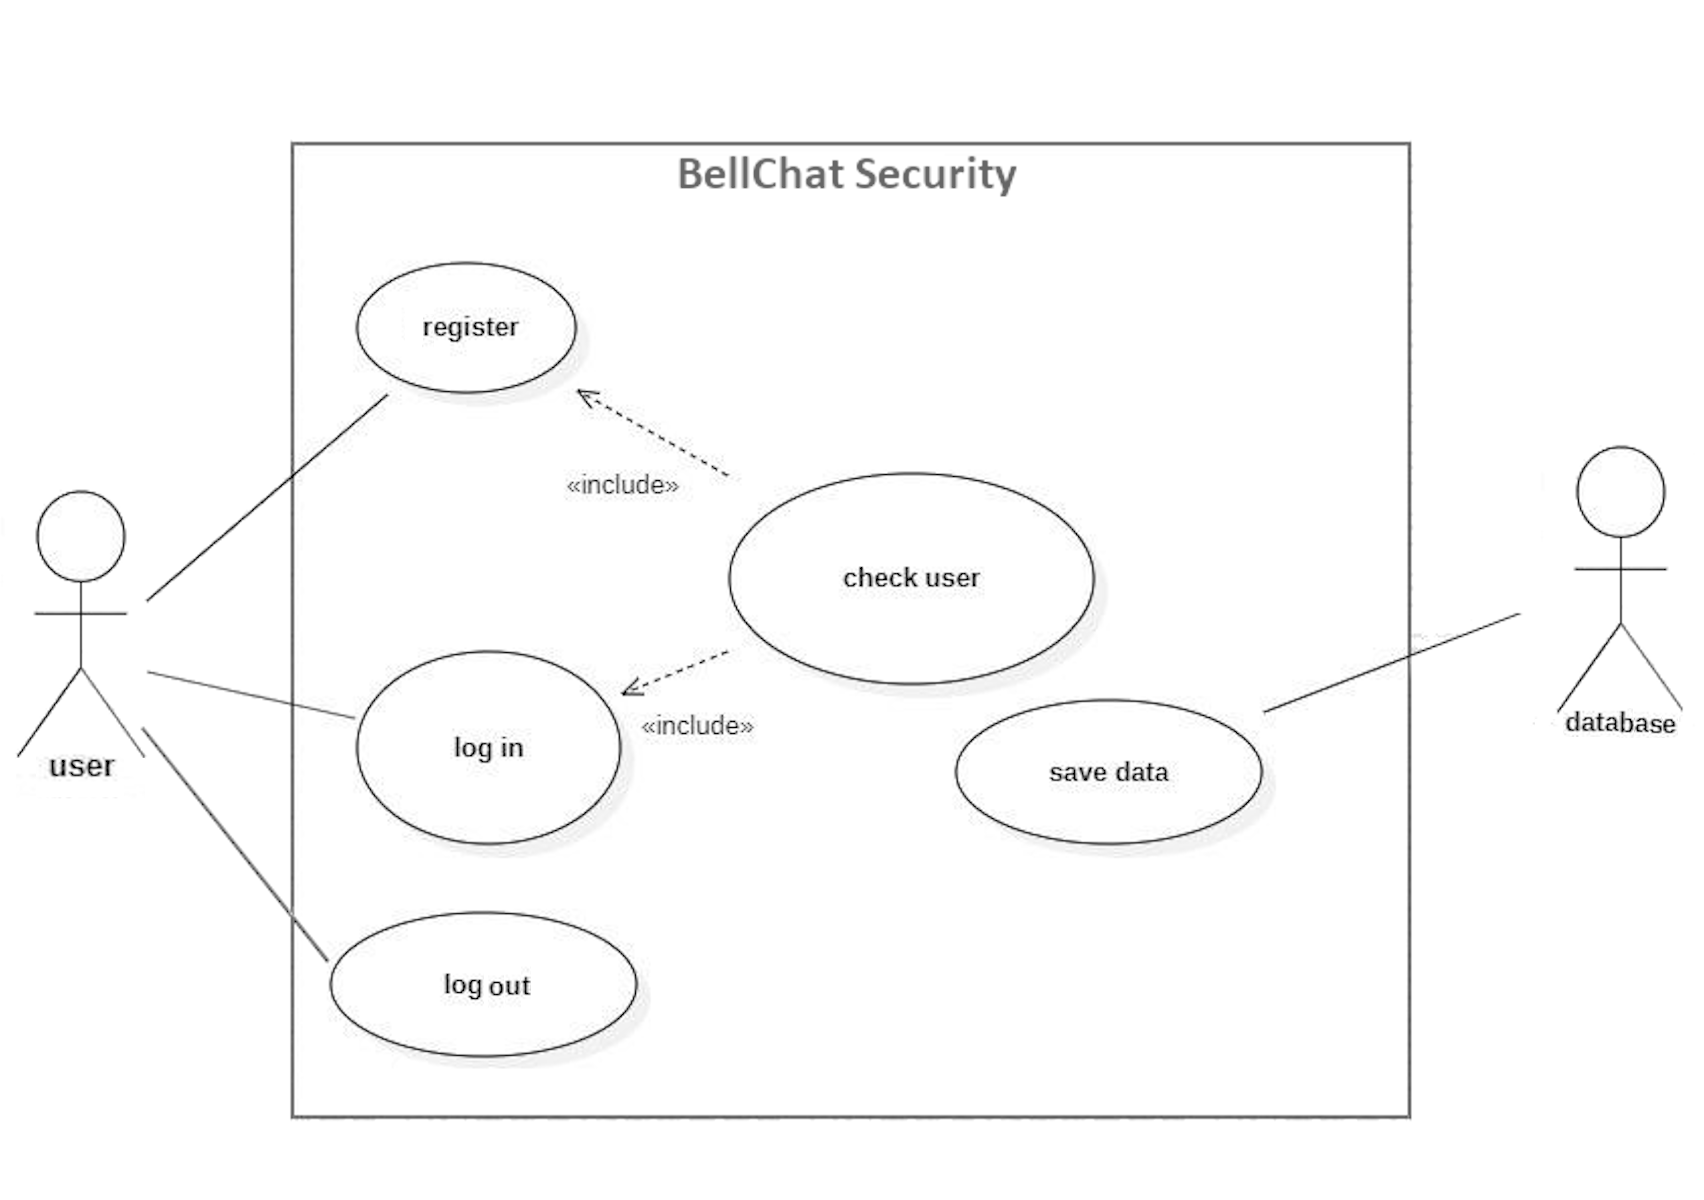
\includegraphics[width=\textwidth]{figures/fig1a.png}
		\caption{BellChat Security-related}
		\label{fig:fig1a}
	\end{subfigure}
	\begin{subfigure}[b]{0.49\textwidth}
		\centering
		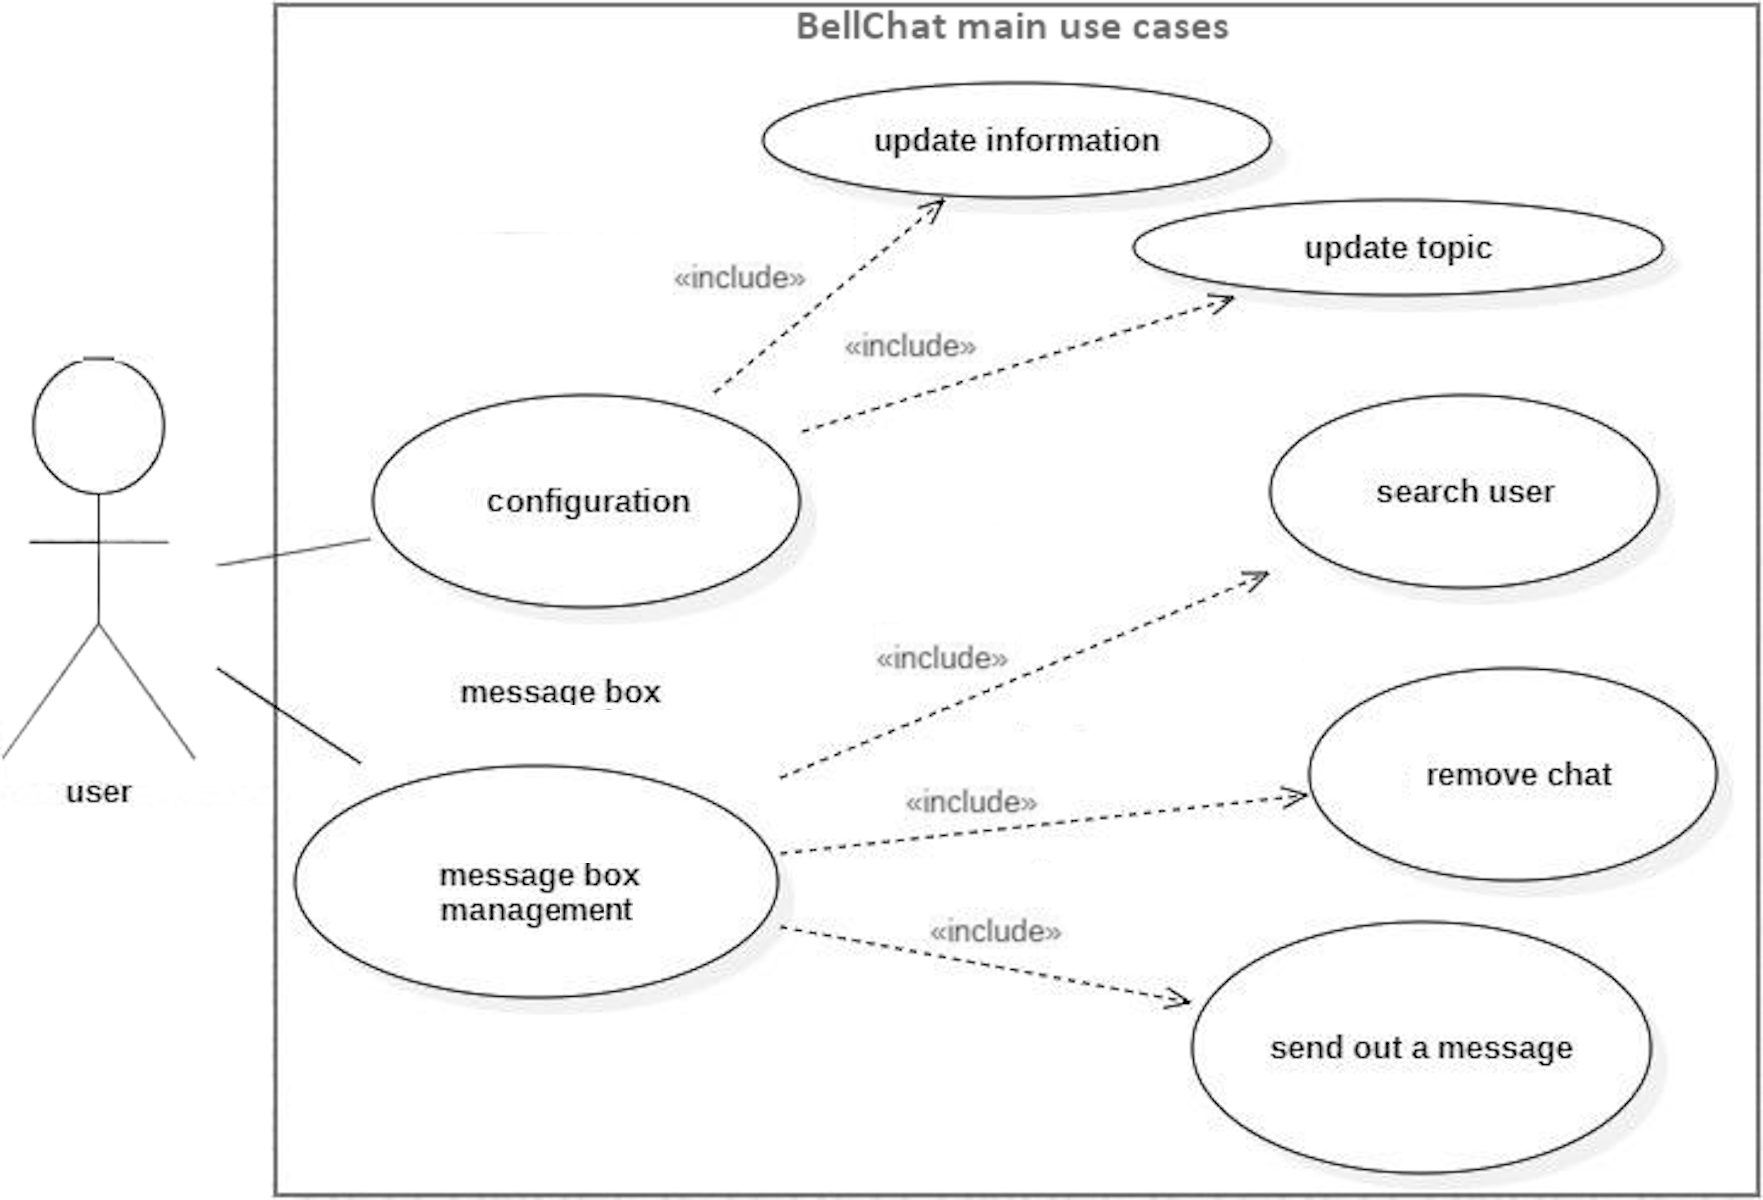
\includegraphics[width=\textwidth]{figures/fig1b.png}
		\caption{BellChat functional requirements}
		\label{fig:fig1b}
	\end{subfigure}
	\caption{BellChat use cases diagram}
	\label{fig:fig1}
\end{figure}

\subsubsection{Use Cases and User Stories} awere used as a tool for eliciting the system requirements

%
\subsection{Autonomous Systems}
%
In this section, we will consider the case when the Hamiltonian $H(x)$
is autonomous. For the sake of simplicity, we shall also assume that it
is $C^{1}$.
We shall first consider the question of nontriviality, within the
general framework of
$\left(A_{\infty},B_{\infty}\right)$-subquadratic Hamiltonians. In
the second subsection, we shall look into the special case when $H$ is
$\left(0,b_{\infty}\right)$-subquadratic,
and we shall try to derive additional information.
%
\subsubsection{The General Case: Nontriviality.}
%
We assume that $H$ is
$\left(A_{\infty},B_{\infty}\right)$-sub\-qua\-dra\-tic at infinity,
for some constant symmetric matrices $A_{\infty}$ and $B_{\infty}$,
with $B_{\infty}-A_{\infty}$ positive definite. Set:
\begin{eqnarray}
\gamma :&=&{\rm smallest\ eigenvalue\ of}\ \ B_{\infty} - A_{\infty} \\
  \lambda : &=& {\rm largest\ negative\ eigenvalue\ of}\ \
  J \frac{d}{dt} +A_{\infty}\ .
\end{eqnarray}
Theorem~\ref{ghou:pre} tells us that if $\lambda +\gamma < 0$, the
boundary-value problem:
\begin{equation}
\begin{array}{rcl}
  \dot{x}&=&JH' (x)\\
  x(0)&=&x (T)
\end{array}
\end{equation}
has at least one solution
$\overline{x}$, which is found by minimizing the dual
action functional:
\begin{equation}
  \psi (u) = \int_{o}^{T} \left[\frac{1}{2}
  \left(\Lambda_{o}^{-1} u,u\right) + N^{\ast} (-u)\right] dt
\end{equation}
on the range of $\Lambda$, which is a subspace $R (\Lambda)_{L}^{2}$
with finite codimension. Here
\begin{equation}
  N(x) := H(x) - \frac{1}{2} \left(A_{\infty} x,x\right)
\end{equation}
is a convex function, and
\begin{equation}
  N(x) \le \frac{1}{2}
  \left(\left(B_{\infty} - A_{\infty}\right) x,x\right)
  + c\ \ \ \forall x\ .
\end{equation}

%
\begin{proposition}
Assume $H'(0)=0$ and $ H(0)=0$. Set:
\begin{equation}
  \delta := \liminf_{x\to 0} 2 N (x) \left\|x\right\|^{-2}\ .
  \label{eq:one}
\end{equation}

If $\gamma < - \lambda < \delta$,
the solution $\overline{u}$ is non-zero:
\begin{equation}
  \overline{x} (t) \ne 0\ \ \ \forall t\ .
\end{equation}
\end{proposition}
%
\begin{proof}
Condition (\ref{eq:one}) means that, for every
$\delta ' > \delta$, there is some $\varepsilon > 0$ such that
\begin{equation}
  \left\|x\right\| \le \varepsilon \Rightarrow N (x) \le
  \frac{\delta '}{2} \left\|x\right\|^{2}\ .
\end{equation}

It is an exercise in convex analysis, into which we shall not go, to
show that this implies that there is an $\eta > 0$ such that
\begin{equation}
  f\left\|x\right\| \le \eta
  \Rightarrow N^{\ast} (y) \le \frac{1}{2\delta '}
  \left\|y\right\|^{2}\ .
  \label{eq:two}
\end{equation}

\begin{figure}
\vspace{2.5cm}
\caption{This is the caption of the figure displaying a white eagle and
a white horse on a snow field}
\end{figure}

Since $u_{1}$ is a smooth function, we will have
$\left\|hu_{1}\right\|_\infty \le \eta$
for $h$ small enough, and inequality (\ref{eq:two}) will hold,
yielding thereby:
\begin{equation}
  \psi (hu_{1}) \le \frac{h^{2}}{2}
  \frac{1}{\lambda} \left\|u_{1} \right\|_{2}^{2} + \frac{h^{2}}{2}
  \frac{1}{\delta '} \left\|u_{1}\right\|^{2}\ .
\end{equation}

If we choose $\delta '$ close enough to $\delta$, the quantity
$\left(\frac{1}{\lambda} + \frac{1}{\delta '}\right)$
will be negative, and we end up with
\begin{equation}
  \psi (hu_{1}) < 0\ \ \ \ \ {\rm for}\ \ h\ne 0\ \ {\rm small}\ .
\end{equation}

On the other hand, we check directly that $\psi (0) = 0$. This shows
that 0 cannot be a minimizer of $\psi$, not even a local one.
So $\overline{u} \ne 0$ and
$\overline{u} \ne \Lambda_{o}^{-1} (0) = 0$. \qed
\end{proof}
%
\begin{corollary}
Assume $H$ is $C^{2}$ and
$\left(a_{\infty},b_{\infty}\right)$-subquadratic at infinity. Let
$\xi_{1},\allowbreak\dots,\allowbreak\xi_{N}$  be the
equilibria, that is, the solutions of $H' (\xi ) = 0$.
Denote by $\omega_{k}$
the smallest eigenvalue of $H'' \left(\xi_{k}\right)$, and set:
\begin{equation}
  \omega : = {\rm Min\,} \left\{\omega_{1},\dots,\omega_{k}\right\}\ .
\end{equation}
If:
\begin{equation}
  \frac{T}{2\pi} b_{\infty} <
  - E \left[- \frac{T}{2\pi}a_{\infty}\right] <
  \frac{T}{2\pi}\omega
  \label{eq:three}
\end{equation}
then minimization of $\psi$ yields a non-constant $T$-periodic solution
$\overline{x}$.
\end{corollary}
%

We recall once more that by the integer part $E [\alpha ]$ of
$\alpha \in \bbbr$, we mean the $a\in \bbbz$
such that $a< \alpha \le a+1$. For instance,
if we take $a_{\infty} = 0$, Corollary 2 tells
us that $\overline{x}$ exists and is
non-constant provided that:

\begin{equation}
  \frac{T}{2\pi} b_{\infty} < 1 < \frac{T}{2\pi}
\end{equation}
or
\begin{equation}
  T\in \left(\frac{2\pi}{\omega},\frac{2\pi}{b_{\infty}}\right)\ .
  \label{eq:four}
\end{equation}

%
\begin{proof}
The spectrum of $\Lambda$ is $\frac{2\pi}{T} \bbbz +a_{\infty}$. The
largest negative eigenvalue $\lambda$ is given by
$\frac{2\pi}{T}k_{o} +a_{\infty}$,
where
\begin{equation}
  \frac{2\pi}{T}k_{o} + a_{\infty} < 0
  \le \frac{2\pi}{T} (k_{o} +1) + a_{\infty}\ .
\end{equation}
Hence:
\begin{equation}
  k_{o} = E \left[- \frac{T}{2\pi} a_{\infty}\right] \ .
\end{equation}

The condition $\gamma < -\lambda < \delta$ now becomes:
\begin{equation}
  b_{\infty} - a_{\infty} <
  - \frac{2\pi}{T} k_{o} -a_{\infty} < \omega -a_{\infty}
\end{equation}
which is precisely condition (\ref{eq:three}).\qed
\end{proof}
%

\begin{lemma}
Assume that $H$ is $C^{2}$ on $\bbbr^{2n} \setminus \{ 0\}$ and
that $H'' (x)$ is non-de\-gen\-er\-ate for any $x\ne 0$. Then any local
minimizer $\widetilde{x}$ of $\psi$ has minimal period $T$.
\end{lemma}
%
\begin{proof}
We know that $\widetilde{x}$, or
$\widetilde{x} + \xi$ for some constant $\xi
\in \bbbr^{2n}$, is a $T$-periodic solution of the Hamiltonian system:
\begin{equation}
  \dot{x} = JH' (x)\ .
\end{equation}

There is no loss of generality in taking $\xi = 0$. So
$\psi (x) \ge \psi (\widetilde{x} )$
for all $\widetilde{x}$ in some neighbourhood of $x$ in
$W^{1,2} \left(\bbbr / T\bbbz ; \bbbr^{2n}\right)$.

But this index is precisely the index
$i_{T} (\widetilde{x} )$ of the $T$-periodic
solution $\widetilde{x}$ over the interval
$(0,T)$, as defined in Sect.~2.6. So
\begin{equation}
  i_{T} (\widetilde{x} ) = 0\ .
  \label{eq:five}
\end{equation}

Now if $\widetilde{x}$ has a lower period, $T/k$ say,
we would have, by Corollary 31:
\begin{equation}
  i_{T} (\widetilde{x} ) =
  i_{kT/k}(\widetilde{x} ) \ge
  ki_{T/k} (\widetilde{x} ) + k-1 \ge k-1 \ge 1\ .
\end{equation}

This would contradict (\ref{eq:five}), and thus cannot happen.\qed
\end{proof}
%
\paragraph{Notes and Comments.}
The results in this section are a
refined version of \cite{smit:wat};
the minimality result of Proposition
14 was the first of its kind.

To understand the nontriviality conditions, such as the one in formula
(\ref{eq:four}), one may think of a one-parameter family
$x_{T}$, $T\in \left(2\pi\omega^{-1}, 2\pi b_{\infty}^{-1}\right)$
of periodic solutions, $x_{T} (0) = x_{T} (T)$,
with $x_{T}$ going away to infinity when $T\to 2\pi \omega^{-1}$,
which is the period of the linearized system at 0.

\begin{table}
\caption{This is the example table taken out of {\it The
\TeX{}book,} p.\,246}
\begin{center}
\begin{tabular}{r@{\quad}rl}
\hline
\multicolumn{1}{l}{\rule{0pt}{12pt}
                   Year}&\multicolumn{2}{l}{World population}\\[2pt]
\hline\rule{0pt}{12pt}
8000 B.C.  &     5,000,000& \\
  50 A.D.  &   200,000,000& \\
1650 A.D.  &   500,000,000& \\
1945 A.D.  & 2,300,000,000& \\
1980 A.D.  & 4,400,000,000& \\[2pt]
\hline
\end{tabular}
\end{center}
\end{table}
%
\begin{theorem} [Ghoussoub-Preiss]\label{ghou:pre}
Assume $H(t,x)$ is
$(0,\varepsilon )$-subquadratic at
infinity for all $\varepsilon > 0$, and $T$-periodic in $t$
\begin{equation}
  H (t,\cdot )\ \ \ \ \ {\rm is\ convex}\ \ \forall t
\end{equation}
\begin{equation}
  H (\cdot ,x)\ \ \ \ \ {\rm is}\ \ T{\rm -periodic}\ \ \forall x
\end{equation}
\begin{equation}
  H (t,x)\ge n\left(\left\|x\right\|\right)\ \ \ \ \
  {\rm with}\ \ n (s)s^{-1}\to \infty\ \ {\rm as}\ \ s\to \infty
\end{equation}
\begin{equation}
  \forall \varepsilon > 0\ ,\ \ \ \exists c\ :\
  H(t,x) \le \frac{\varepsilon}{2}\left\|x\right\|^{2} + c\ .
\end{equation}

Assume also that $H$ is $C^{2}$, and $H'' (t,x)$ is positive definite
everywhere. Then there is a sequence $x_{k}$, $k\in \bbbn$, of
$kT$-periodic solutions of the system
\begin{equation}
  \dot{x} = JH' (t,x)
\end{equation}
such that, for every $k\in \bbbn$, there is some $p_{o}\in\bbbn$ with:
\begin{equation}
  p\ge p_{o}\Rightarrow x_{pk} \ne x_{k}\ .
\end{equation}
\qed
\end{theorem}
%
\begin{example} [{{\rm External forcing}}]
Consider the system:
\begin{equation}
  \dot{x} = JH' (x) + f(t)
\end{equation}
where the Hamiltonian $H$ is
$\left(0,b_{\infty}\right)$-subquadratic, and the
forcing term is a distribution on the circle:
\begin{equation}
  f = \frac{d}{dt} F + f_{o}\ \ \ \ \
  {\rm with}\ \ F\in L^{2} \left(\bbbr / T\bbbz; \bbbr^{2n}\right)\ ,
\end{equation}
where $f_{o} : = T^{-1}\int_{o}^{T} f (t) dt$. For instance,
\begin{equation}
  f (t) = \sum_{k\in \bbbn} \delta_{k} \xi\ ,
\end{equation}
where $\delta_{k}$ is the Dirac mass at $t= k$ and
$\xi \in \bbbr^{2n}$ is a
constant, fits the prescription. This means that the system
$\dot{x} = JH' (x)$ is being excited by a
series of identical shocks at interval $T$.
\end{example}
%
\begin{definition}
Let $A_{\infty} (t)$ and $B_{\infty} (t)$ be symmetric
operators in $\bbbr^{2n}$, depending continuously on
$t\in [0,T]$, such that
$A_{\infty} (t) \le B_{\infty} (t)$ for all $t$.

A Borelian function
$H: [0,T]\times \bbbr^{2n} \to \bbbr$
is called
$\left(A_{\infty} ,B_{\infty}\right)$-{\it subquadratic at infinity}
if there exists a function $N(t,x)$ such that:
\begin{equation}
  H (t,x) = \frac{1}{2} \left(A_{\infty} (t) x,x\right) + N(t,x)
\end{equation}
\begin{equation}
  \forall t\ ,\ \ \ N(t,x)\ \ \ \ \
  {\rm is\ convex\ with\  respect\  to}\ \ x
\end{equation}
\begin{equation}
  N(t,x) \ge n\left(\left\|x\right\|\right)\ \ \ \ \
  {\rm with}\ \ n(s)s^{-1}\to +\infty\ \ {\rm as}\ \ s\to +\infty
\end{equation}
\begin{equation}
  \exists c\in \bbbr\ :\ \ \ H (t,x) \le
  \frac{1}{2} \left(B_{\infty} (t) x,x\right) + c\ \ \ \forall x\ .
\end{equation}

If $A_{\infty} (t) = a_{\infty} I$ and
$B_{\infty} (t) = b_{\infty} I$, with
$a_{\infty} \le b_{\infty} \in \bbbr$,
we shall say that $H$ is
$\left(a_{\infty},b_{\infty}\right)$-subquadratic
at infinity. As an example, the function
$\left\|x\right\|^{\alpha}$, with
$1\le \alpha < 2$, is $(0,\varepsilon )$-subquadratic at infinity
for every $\varepsilon > 0$. Similarly, the Hamiltonian
\begin{equation}
H (t,x) = \frac{1}{2} k \left\|k\right\|^{2} +\left\|x\right\|^{\alpha}
\end{equation}
is $(k,k+\varepsilon )$-subquadratic for every $\varepsilon > 0$.
Note that, if $k<0$, it is not convex.
\end{definition}
%

\paragraph{Notes and Comments.}
The first results on subharmonics were
obtained by Rabinowitz in \cite{fo:kes:nic:tue}, who showed the existence of
infinitely many subharmonics both in the subquadratic and superquadratic
case, with suitable growth conditions on $H'$. Again the duality
approach enabled Clarke and Ekeland in \cite{may:ehr:stein} to treat the
same problem in the convex-subquadratic case, with growth conditions on
$H$ only.

Recently, Michalek and Tarantello (see \cite{fost:kes} and \cite{czaj:fitz})
have obtained lower bound on the number of subharmonics of period $kT$,
based on symmetry considerations and on pinching estimates, as in
Sect.~5.2 of this article.

%
% ---- Bibliography ----
%

\begin{thebibliography}{6}
\printbibliography

%\bibitem {smit:wat}
%Smith, T.F., Waterman, M.S.: Identification of common molecular subsequences.
%J. Mol. Biol. 147, 195?197 (1981). \url{doi:10.1016/0022-2836(81)90087-5}

%\bibitem {may:ehr:stein}
%May, P., Ehrlich, H.-C., Steinke, T.: ZIB structure prediction pipeline:
%composing a complex biological workflow through web services.
%In: Nagel, W.E., Walter, W.V., Lehner, W. (eds.) Euro-Par 2006.
%LNCS, vol. 4128, pp. 1148?1158. Springer, Heidelberg (2006).
%\url{doi:10.1007/11823285_121}

%\bibitem {fost:kes}
%Foster, I., Kesselman, C.: The Grid: Blueprint for a New Computing Infrastructure.
%Morgan Kaufmann, San Francisco (1999)

%\bibitem {czaj:fitz}
%Czajkowski, K., Fitzgerald, S., Foster, I., Kesselman, C.: Grid information services
%for distributed resource sharing. In: 10th IEEE International Symposium
%on High Performance Distributed Computing, pp. 181?184. IEEE Press, New York (2001).
%\url{doi: 10.1109/HPDC.2001.945188}

%\bibitem {fo:kes:nic:tue}
%Foster, I., Kesselman, C., Nick, J., Tuecke, S.: The physiology of the grid: an open grid services architecture for distributed systems integration. Technical report, Global Grid
%Forum (2002)

%\bibitem {onlyurl}
%National Center for Biotechnology Information. \url{http://www.ncbi.nlm.nih.gov}

\end{thebibliography}
\end{document}
